%%%%%%%%%%%%%%%%%%%%%%%%%%%%%%%%%%%%%%%%%%%%%%
%                insertmeeting
% 1) Title (something creative & funny?)
% 2) Date (MM/DD/YYYY)
% 3) Location (ex. Hagerty High School)
% 4) People/Committees Present 
% 5) Picture 
% 6) Start Time & Stop Time (ex. 12:30AM to 4:30PM)
%%%%%%%%%%%%%%%%%%%%%%%%%%%%%%%%%%%%%%%%%%%%%%
\insertmeeting 
	{Woah, Worlds!} 
	{04/14/22} 
	{Hagerty High School}
	{James, Jensen, Nathan, Ritam}
	{Images/RobotPics/robot.jpg}
	{2:30 - 6:30}
	
\hhscommittee{General}
\noindent\hfil\rule{\textwidth}{.4pt}\hfil
\subsubsection*{Goals}
\begin{itemize}
    \item Prepare for Worlds
    \item Check all members' forms
    \item Discuss housing, food, and travel plans.

\end{itemize} 

\noindent\hfil\rule{\textwidth}{.4pt}\hfil

\subsubsection*{Accomplishments}
Today we held a team-wide meeting to discuss worlds. First, we checked to ensure that all members submitted travel payments and the required forms to take 4 days off school. Since all the paperwork was finished, we could move onto the next step. We plan to leave on 4/19 and return on 4/24. We plan to be staying at the Mariott Medical Center in Houston. Our team agreed on a dress code and discussed the meal plans for each day we are in Houston. We also received the flight information. We are nervous yet excited to have fun in Houston. We also began writing packing lists, printing out our flyers and other materials, and making buttons. A team member also created Florida-shaped pins using our Glowforge laser cutter to hand out to other teams at Worlds. 

\begin{figure}[htp]
\centering
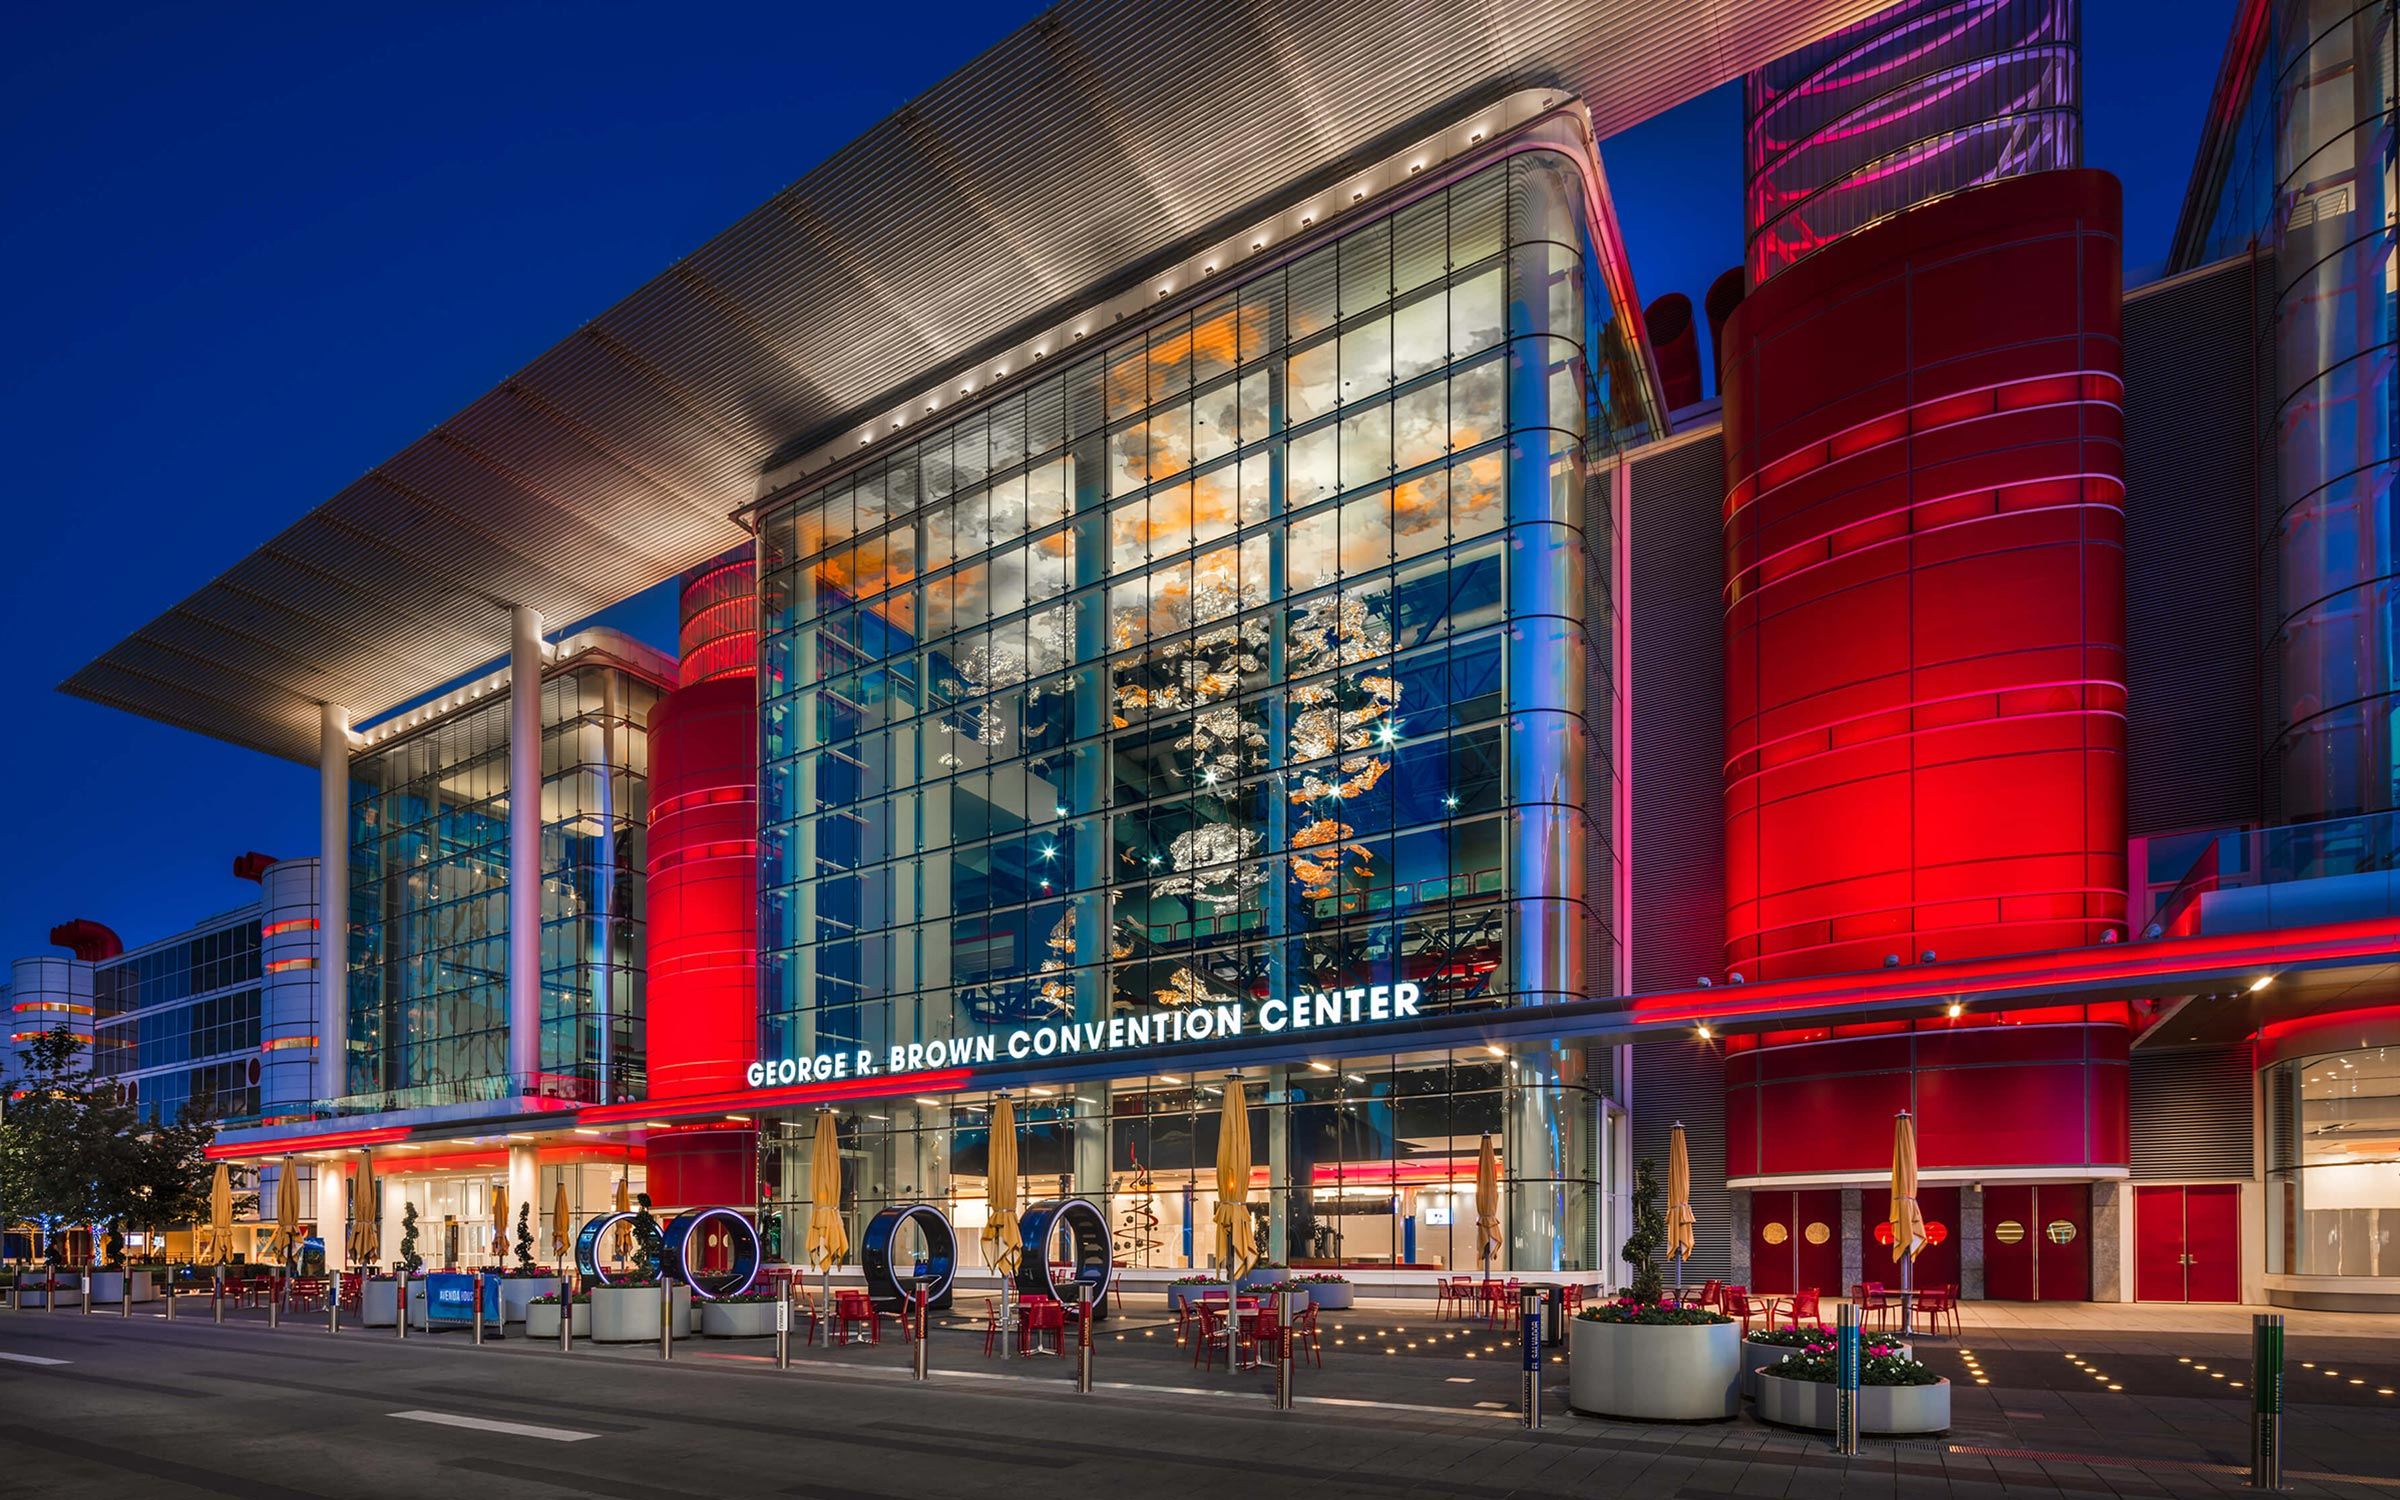
\includegraphics[width=0.95\textwidth, angle=0]{Meetings/April/04-14-22/04-14-22 1.JPG}
\caption{The George R Brown Convention Center, where we will be competing.}
\label{fig:041422_1}
\end{figure}

\whatsnext{
\begin{itemize}
    \item Begin packing for Worlds
    \item Finish robot autonomous
    \item Manufacture extra parts (Intake plates, team elements, etc)
\end{itemize} 
}

